%--------------- Personalize your document here ---------------
\author{Messaoud HAMDI}
\newcommand{\supervisorone}{Pierre MIRAT} % Enter your supervisor's name

\title{Implémentation d'une plateforme de tests automatisés avec Cucumber pour le projet COTS SNCF\\[0.5 cm]} %Enter the title of your report 
\date{2025 - 2026} % insert a specific date	

\documentclass[a4paper,12pt,twoside]{report}
\setcounter{secnumdepth}{3}
\setlength{\parindent}{20pt}
\usepackage[left=25mm,top=25mm,right=25mm,bottom=25mm]{geometry}
\usepackage{gensymb}
\usepackage{etoolbox} %required for cover page
\usepackage{booktabs}
\usepackage[table,xcdraw]{xcolor}
\usepackage[usestackEOL]{stackengine}
\usepackage[T1]{fontenc}
\usepackage[utf8]{inputenc}
\usepackage{bm}
\usepackage{graphicx}
\usepackage{subcaption}
\usepackage{amsfonts}
\usepackage{mathtools}
\usepackage[user,titleref]{zref}
\usepackage{xcolor}
\definecolor{mauve}{rgb}{0.58,0,0.82}
\definecolor{dkgreen}{rgb}{0,0.6,0}
\usepackage{float}
\usepackage[hyphens]{url}
\usepackage{hyperref}
\usepackage{multirow}
\usepackage[capitalise]{cleveref}
\usepackage{enumitem,kantlipsum}
\usepackage{amssymb}
\usepackage[ruled,vlined]{algorithm2e}
\usepackage{listings}
\usepackage{minted}
\usepackage{setspace}
\usepackage{afterpage}
\usepackage{titlesec}
\usepackage[section]{placeins}
\usepackage{diagbox}
\usepackage{fancyhdr}
\usepackage{tabularx}
\usepackage{longtable}
\usepackage{indentfirst}
\usepackage{lettrine}
\usepackage{pdfpages}
\usepackage{tcolorbox}
\newcommand{\ts}{\textsuperscript}
\usepackage[tableposition = top]{caption}
\usepackage[nottoc]{tocbibind} % This package automatically includes lists in TOC

\usepackage{placeins}

% ENHANCED BULLET POINT CONFIGURATION
% Force visible bullet points with multiple fallback options
\usepackage{textcomp}
\usepackage{pifont}

% Define custom bullet symbols that are guaranteed to show
\newcommand{\bulletone}{\textbullet}
\newcommand{\bullettwo}{--}
\newcommand{\bulletthree}{*}

% Override default itemize labels with visible symbols
\renewcommand{\labelitemi}{\bulletone}
\renewcommand{\labelitemii}{\bullettwo}
\renewcommand{\labelitemiii}{\bulletthree}

% Enhanced itemize settings with guaranteed visibility
\setlist[itemize,1]{label=\bulletone, leftmargin=2em, itemsep=0.4em, parsep=0.2em, topsep=0.5em}
\setlist[itemize,2]{label=\bullettwo, leftmargin=2.5em, itemsep=0.3em, parsep=0.1em}
\setlist[itemize,3]{label=\bulletthree, leftmargin=3em, itemsep=0.2em, parsep=0.1em}
\setlist[enumerate,1]{leftmargin=2em, itemsep=0.4em, parsep=0.2em, topsep=0.5em}
\setlist[description]{leftmargin=2em, itemsep=0.4em, parsep=0.2em, topsep=0.5em}

% Better spacing for sections
\titlespacing{\chapter}{0pt}{-30pt}{20pt}
\titlespacing{\section}{0pt}{12pt}{6pt}
\titlespacing{\subsection}{0pt}{10pt}{4pt}

\usemintedstyle{emacs}
\newcommand\blankpage{%
    \null
    \thispagestyle{empty}%
    \addtocounter{page}{-1}%
    \newpage}

% Proper line spacing
\renewcommand{\baselinestretch}{1.2}

\hypersetup{
    colorlinks=true,
    linkcolor={black},
    citecolor={blue!50!black},
    urlcolor={blue!80!black},
    bookmarksnumbered=true,
    pdfstartview=FitH
}

\linespread{1.15}

\newtheorem{theorem}{Theorem}[section]
\graphicspath{{figures/}}	

% Enhanced quote environment
\usepackage{xcolor}
\definecolor{quotemark}{gray}{0.7}
\makeatletter
\def\fquote{%
    \@ifnextchar[{\fquote@i}{\fquote@i[]}%]
           }%
\def\fquote@i[#1]{%
    \def\tempa{#1}%
    \@ifnextchar[{\fquote@ii}{\fquote@ii[]}%]
                 }%
\def\fquote@ii[#1]{%
    \def\tempb{#1}%
    \@ifnextchar[{\fquote@iii}{\fquote@iii[]}%]
                      }%
\def\fquote@iii[#1]{%
    \def\tempc{#1}%
    \vspace{1em}%
    \noindent%
    \begin{list}{}{%
         \setlength{\leftmargin}{0.02\textwidth}%
         \setlength{\rightmargin}{0.02\textwidth}%
                  }%
         \item[]%
         \begin{picture}(0,0)%
         \put(-15,-5){\makebox(0,0){\scalebox{3}{\textcolor{quotemark}{``}}}}%
         \end{picture}%
         \begingroup\itshape}%
 %%%%********************************************************************
 \def\endfquote{%
 \endgroup\par%
 \makebox[0pt][l]{%
 \hspace{0.8\textwidth}%
 \begin{picture}(0,0)(0,0)%
 \put(15,15){\makebox(0,0){%
 \scalebox{3}{\color{quotemark}''}}}%
 \end{picture}}%
 \ifx\tempa\empty%
 \else%
    \ifx\tempc\empty%
       \hfill\rule{100pt}{0.5pt}\\\mbox{}\hfill\tempa,\ \emph{\tempb}%
   \else%
       \hfill\rule{100pt}{0.5pt}\\\mbox{}\hfill\tempa,\ \emph{\tempb},\ \tempc%
   \fi\fi\par%
   \vspace{0.5em}%
 \end{list}%
 }%
 \makeatother

% Fix headheight warning
\setlength{\headheight}{14.5pt}

% Page header and footer setup
\pagestyle{fancy}
\fancyhf{}
\renewcommand{\headrulewidth}{0.4pt}
\fancyhead[LE,RO]{\thepage}
\fancyhead[LO]{\nouppercase{\rightmark}}
\fancyhead[RE]{\nouppercase{\leftmark}}

\begin{document}

\pagenumbering{roman}
\thispagestyle{empty}
\begin{titlepage}
  \newcommand{\HRule}{\rule{\linewidth}{0.5mm}} % Defines a new command for the horizontal lines, change thickness here
  \center % Center everything on the page
  %----------------------------------------------------------------------------------------
  %	HEADING SECTIONS
  %----------------------------------------------------------------------------------------
  % Adjusting the layout to place logos side by side
  \begin{minipage}{0.32\textwidth}
      \centering
      
\includegraphics[scale=0.22]{figures/soprasteria.png}
  \end{minipage}
  \hfill
  \begin{minipage}{0.32\textwidth}
      \centering
      
\includegraphics[scale=0.2]{figures/IMTA.png}
  \end{minipage}
  \vspace{15mm}
  \begin{center}
  {\large \bfseries Diplôme d'Ingénieur Généraliste}\\[0.5cm]
  {\large Filière : Génie Logiciel et Innovation (LOGIN)}\\[0.8cm]
  {\huge \bfseries Rapport de Stage de Fin d'Études}\\
  \end{center}
  \vspace{7mm}
  % Title
  \rule{\linewidth}{0.3mm} \\[0.4cm]
  { \huge \bfseries Implémentation d'une plateforme de tests automatisés avec Cucumber pour le projet COTS SNCF\\[0.4cm] }
  \rule{\linewidth}{0.3mm} \\[1cm]
  \vspace{5mm}
  \noindent
  \begin{minipage}{0.5\textwidth}
    \begin{flushleft} \large
      \emph{Auteur :}\\
      \vskip 0.05cm
      \textsc{Messaoud HAMDI}\\
      \small{\href{mailto:messaoud.hamdi@imt-atlantique.net}{messaoud.hamdi@imt-atlantique.net}}\\[0.5cm]
    \end{flushleft}
  \end{minipage}
  \begin{minipage}{0.4\textwidth}
    \begin{flushright} \large
      \begin{flushleft}
      \emph{Encadrants :} \\
      \vskip 0.05cm
      M. \textsc{Pierre MIRAT}\\
      \small{\href{mailto:pierre.mirat@soprasteria.com}{pierre.mirat@soprasteria.com}}\\[0.5cm]
      
       \large Mme. \textsc{Hélène COULLON}\\
      \small{\href{mailto:helene.coullon@imt-atlantique.fr}{helene.coullon@imt-atlantique.fr}}\\[0.5cm]
      \end{flushleft}
    \end{flushright}
  \end{minipage}\\[1cm]
  \large \emph{Travail effectué du 1er avril 2025 au 31 août 2025 chez :}\\[0.5cm]
  \textbf{Sopra Steria}
  \vfill
  \begin{flushleft}
  \begin{center}
  {\large Année Universitaire : 2025 - 2026}
  \end{center}
  \end{flushleft}
  
\includegraphics[scale=0.4]{figures/IMTA_large.png}
  \end{titlepage}
\newpage

\addtocontents{toc}{\protect\setcounter{tocdepth}{-1}} % Exclude next sections from TOC
\chapter*{Dédicace}
\addcontentsline{toc}{chapter}{Dédicace}
\begin{fquote}
\begin{center}
\large{
\uppercase{À} tous ceux qui illuminent mon existence et nourrissent mon cœur, \\[12pt]
\uppercase{À} ma précieuse mère Mahjouba pour son amour infini, sa bienveillance et ses sacrifices innombrables,\\
\uppercase{À} la mémoire éternelle de mon père bien-aimé dont l'héritage de courage et de sagesse continue de m'éclairer, \\
\uppercase{À} tous mes frères et sœurs qui apportent lumière et réconfort à chaque étape de mon parcours, \\
\uppercase{À} mes amis fidèles pour leur présence chaleureuse et tous les instants précieux partagés ensemble,\\
\uppercase{À} mes collègues de Sopra Steria qui m'ont accueilli avec générosité et ont partagé leur expertise,\\
\uppercase{À} mes professeurs d'IMT Atlantique qui ont enrichi mon apprentissage et façonné ma vision d'ingénieur,\\
\uppercase{E}nfin, à tous ceux qui œuvrent dans l'ombre, créant l'environnement propice à ma formation et à mon épanouissement,\\[12pt]
Ce modeste travail témoigne de ma reconnaissance envers vous tous. Merci.
}
\end{center}
\bigskip
\medskip
\end{fquote}
\hspace*{\fill} \textbf{\textit{\large{-Messaoud}}}
\clearpage
\newpage
\chapter*{Remerciements}
\addcontentsline{toc}{chapter}{Remerciements} 
\lettrine{\textbf{E}}\lowercase{n} témoignage de ma reconnaissance sincère, je souhaite exprimer ma profonde gratitude à toutes les personnes qui ont joué un rôle déterminant dans la réalisation de mon projet de stage chez Sopra Steria. \\[0.3cm]
\\
En premier lieu, je tiens à remercier chaleureusement ma tutrice académique, \textbf{Mme Hélène Coullon}, pour son accompagnement depuis le début de mon apprentissage. Ses conseils éclairés et son soutien constant ont été précieux tout au long de cette aventure. \\[0.3cm]
\\
Je souhaite également adresser mes remerciements les plus sincères à mon maître de stage, \textbf{M. Pierre Mirat}, pour m'avoir offert cette opportunité exceptionnelle chez Sopra Steria et pour son encadrement attentif tout au long du projet COTS. Son expertise métier et sa vision stratégique ont grandement enrichi mon approche de ce travail. \\[0.3cm]
\\
J'exprime une gratitude particulière envers \textbf{M. Tom Richardson}, le Tech Lead, qui m'a constamment guidé dans les défis techniques et m'a apporté un soutien inestimable pour surmonter les problématiques complexes. Son savoir-faire technique a été fondamental dans mon processus d'apprentissage. \\[0.3cm]
\\
Un remerciement spécial s'adresse à mes collègues \textbf{Louis Legendre} et \textbf{Mélina Loyant} pour leur collaboration fructueuse, leurs conseils avisés et leur soutien durant toute la durée du projet. Leur disponibilité et leur volonté de partager leurs connaissances ont facilité mon intégration et enrichi mon expérience. \\[0.3cm]
\\
Par ailleurs, je souhaite exprimer ma reconnaissance aux analystes métier, \textbf{Florian Carré} et \textbf{Marie-Émilie Deschez}, qui m'ont fourni des éclairages essentiels sur les enjeux business et m'ont aidé à comprendre les exigences fonctionnelles du projet COTS. Leur expertise dans la traduction des besoins métier en spécifications techniques a été cruciale pour le succès de l'implémentation de la plateforme de tests. \\[0.3cm] 
\\
Enfin, je tiens à remercier les membres du jury pour le temps qu'ils consacrent à l'analyse critique de mon travail et pour leur expertise dans l'évaluation de ce projet.
\newpage
\chapter*{Résumé}
%\addcontentsline{toc}{chapter}{Résumé}

\lettrine{\textbf{C}}\lowercase{e} rapport présente les travaux réalisés chez Sopra Steria dans le cadre du stage de fin d'études, portant sur la conception et l'implémentation d'un framework d'automatisation des tests pour le projet SNCF COTS (Catalogue des Offres de Transport et de Services). Cette mission d'ingénierie complexe vise à transformer radicalement les processus d'assurance qualité d'un système critique par l'automatisation intelligente des tests de régression.

Le défi technique principal consiste à concevoir une solution d'automatisation native pour une architecture microservices distribuée, intégrant les principes du Behavior-Driven Development (BDD) via Cucumber avec l'écosystème Spring Boot existant. Cette innovation méthodologique résout la problématique de validation exhaustive de neuf services critiques tout en maintenant l'expressivité métier nécessaire à la collaboration avec les analystes fonctionnels.

L'approche d'ingénieur adoptée s'articule autour d'une méthodologie rigoureuse comprenant l'analyse systémique de l'architecture existante, la conception d'une solution modulaire et évolutive, l'implémentation de mécanismes de robustesse avancés et l'intégration transparente dans le pipeline CI/CD Jenkins. Cette démarche assure une transformation contrôlée des processus avec validation continue des performances et de la fiabilité.

Les résultats quantitatifs confirment l'efficacité de la solution développée : réduction de 85% des temps de validation (de 8 heures à 1h15), amélioration de la fiabilité à 94% avec moins de 2% de faux positifs, et augmentation de 40% de la couverture fonctionnelle. Ces performances valident l'approche technique et démontrent la création de valeur opérationnelle significative.

L'analyse multidimensionnelle révèle des impacts dépassant largement le cadre technique initial. La dimension organisationnelle illustre la transformation des pratiques de travail et l'évolution des rôles professionnels. La dimension environnementale et sociétale confirme la contribution à la durabilité numérique et à l'amélioration du service public ferroviaire. La dimension stratégique et économique démontre un retour sur investissement de 350% sur cinq ans et une différenciation concurrentielle pour Sopra Steria.

Cette mission valide l'acquisition des compétences d'ingénieur selon le référentiel IMT Atlantique, démontrant la capacité d'analyse de problématiques complexes, de conception de solutions innovantes, de prise de décision éclairée et d'intégration des enjeux sociétaux dans l'exercice du métier d'ingénieur.

\\[0.3cm]
\\
\rule{\linewidth}{0.2mm} \\[0.2cm]
\textbf {Mots-clés :} automatisation des tests, framework Cucumber, architecture microservices, BDD, CI/CD, Jenkins, Spring Boot, assurance qualité, transformation numérique, SNCF COTS, ingénierie logicielle, DevOps. \\
\rule{\linewidth}{0.2mm}
\newpage
\chapter*{Acronymes}
\addcontentsline{toc}{chapter}{Acronymes}
\begin{description}
    \item[SNCF] \hfill Société Nationale des Chemins de fer Français
    \item[COTS] \hfill Catalogue des Offres de Transport et de Services
    \item[BDD] \hfill Développement Piloté par le Comportement (Behavior-Driven Development)
    \item[TDD] \hfill Développement Piloté par les Tests (Test-Driven Development)
    \item[CI/CD] \hfill Intégration Continue/Déploiement Continu (Continuous Integration/Continuous Deployment)
    \item[API] \hfill Interface de Programmation d'Application (Application Programming Interface)
    \item[REST] \hfill Transfert d'État Représentationnel (Representational State Transfer)
    \item[JSON] \hfill Notation d'Objet JavaScript (JavaScript Object Notation)
    \item[HTTP] \hfill Protocole de Transfert HyperTexte (HyperText Transfer Protocol)
    \item[JVM] \hfill Machine Virtuelle Java (Java Virtual Machine)
    \item[JDK] \hfill Kit de Développement Java (Java Development Kit)
    \item[IDE] \hfill Environnement de Développement Intégré (Integrated Development Environment)
    \item[UI] \hfill Interface Utilisateur (User Interface)
    \item[UAT] \hfill Tests d'Acceptation Utilisateur (User Acceptance Testing)
    \item[QA] \hfill Assurance Qualité (Quality Assurance)
    \item[DevOps] \hfill Développement et Opérations (Development and Operations)
    \item[SCM] \hfill Gestion du Code Source (Source Code Management)
    \item[MVP] \hfill Produit Minimum Viable (Minimum Viable Product)
\end{description>
\newpage

\addtocontents{toc}{\protect\setcounter{tocdepth}{3}} % Re-include sections in TOC
\renewcommand{\contentsname}{Table des matières} 
\tableofcontents{}
\newpage

\renewcommand{\listfigurename}{Liste des figures}
\listoffigures
\newpage

\renewcommand{\listtablename}{Liste des tableaux}
\listoftables
\clearpage

\newpage
\pagenumbering{arabic}% Arabic page numbers (and reset to 1)
% ========================================================================
% INTRODUCTION GÉNÉRALE MISE À JOUR
% ========================================================================

\chapter*{Introduction générale}
\addcontentsline{toc}{chapter}{Introduction générale}

\lettrine{\textbf{L}}\lowercase{a} transformation numérique des systèmes critiques constitue un défi majeur pour les organisations modernes, particulièrement dans le secteur ferroviaire où la fiabilité, la performance et la sécurité sont impératives. Dans ce contexte, la Société Nationale des Chemins de fer Français (SNCF) s'engage dans une modernisation ambitieuse de son système d'information à travers le projet COTS (Catalogue des Offres de Transport et de Services). Cette initiative stratégique, menée en partenariat avec Sopra Steria, vise à créer un référentiel unifié remplaçant les multiples systèmes patrimoniaux disparates, impactant directement l'expérience de millions de voyageurs quotidiennement et les processus opérationnels critiques du transport ferroviaire français.

Face à la complexité croissante de l'écosystème COTS, composé de neuf microservices critiques interconnectés dans une architecture distribuée moderne, l'assurance qualité représente un enjeu stratégique et technique majeur. Les processus actuels de tests de non-régression, réalisés manuellement via l'outil ALM, génèrent des cycles de validation de huit heures et mobilisent intensivement les équipes qualité sur des tâches répétitives à faible valeur ajoutée. Cette problématique s'intensifie avec l'accélération des cycles de développement agiles, la nécessité d'intégrer des pratiques de livraison continue et l'impératif de maintenir des standards de qualité rigoureux pour un système ferroviaire où toute défaillance peut avoir des conséquences opérationnelles critiques.

\textbf{L'enjeu principal de cette mission de stage} consiste donc à concevoir et implémenter une solution d'automatisation complète et innovante des tests de régression pour le projet COTS. Cette mission d'ingénieur s'articule autour de la création d'un framework de tests automatisés utilisant l'approche Behavior-Driven Development (BDD) avec Cucumber, intégré nativement à l'architecture Spring Boot existante, et l'orchestration de cette solution dans le pipeline CI/CD Jenkins. L'objectif est de transformer fondamentalement les pratiques d'assurance qualité en réduisant drastiquement les temps d'exécution des campagnes de test (objectif de réduction de 80\%) tout en améliorant significativement leur fiabilité, leur reproductibilité et leur expressivité métier.

Cette problématique technique complexe nécessite une approche d'ingénieur rigoureuse et multidimensionnelle. Sur le plan technique et scientifique, elle implique la maîtrise des frameworks de test modernes, la conception d'architectures d'automatisation robustes, l'implémentation de mécanismes de gestion de la complexité et l'intégration harmonieuse dans des environnements de production critiques. Sur le plan organisationnel, elle requiert une compréhension approfondie des impacts sur les équipes de développement et d'assurance qualité, des processus de conduite du changement et de l'évolution des pratiques professionnelles. Les dimensions environnementale et sociétale touchent à l'optimisation des ressources informatiques, la réduction de l'empreinte carbone numérique et l'amélioration de la qualité des services ferroviaires contribuant au transport durable. Enfin, l'analyse stratégique et économique porte sur la valeur ajoutée pour Sopra Steria, l'impact économique pour la SNCF et les enjeux concurrentiels du secteur ferroviaire en transformation.

Le choix de ce stage s'inscrit pleinement dans mon projet professionnel d'ingénieur spécialisé en développement logiciel, DevOps et ingénierie de la qualité. Cette mission offre l'opportunité unique de travailler sur un projet d'innovation technique à fort impact sociétal, tout en développant une expertise approfondie des systèmes critiques, des architectures microservices et des pratiques d'assurance qualité modernes. L'environnement technologique avancé de Sopra Steria, la complexité du projet COTS et la collaboration avec des experts métier ferroviaires constituent un cadre d'apprentissage exceptionnel pour acquérir les compétences d'ingénieur recherchées dans le secteur de la transformation numérique et développer une vision systémique des enjeux de l'ingénierie logicielle contemporaine.

Ce rapport structure l'analyse de cette mission d'ingénieur en quatre chapitres progressifs et complémentaires. Le \textbf{premier chapitre} présente le contexte professionnel chez Sopra Steria et détaille le projet COTS dans son environnement technique, stratégique et organisationnel, établissant les fondements nécessaires à la compréhension des enjeux multidimensionnels. Le \textbf{deuxième chapitre} expose la conception et la réalisation du framework d'automatisation, depuis l'analyse systémique des problématiques jusqu'à l'implémentation complète des solutions techniques et leur intégration CI/CD, incluant l'évaluation critique des résultats obtenus. Le \textbf{troisième chapitre} développe l'analyse multidimensionnelle requise pour une formation d'ingénieur, examinant successivement les dimensions technique et scientifique, organisationnelle, environnementale et sociétale, ainsi que stratégique et économique du projet, révélant les impacts complexes de cette innovation technique. Le \textbf{chapitre final} propose une analyse critique approfondie de l'expérience d'ingénieur, évaluant la pertinence des approches méthodologiques employées, les compétences développées et transférables, et offrant des perspectives d'évolution professionnelle ainsi que des recommandations stratégiques pour l'entreprise et le secteur.
\newpage
\chapter{Contexte et cadre du projet}

\section{Introduction}

Ce premier chapitre présente une vue d'ensemble du stage en exposant l'entreprise d'accueil et le contexte du projet COTS. Il établit le cadre contextuel nécessaire à la compréhension des enjeux multidimensionnels de cette mission de fin d'études, centrée sur un défi d'ingénierie complexe : la conception et l'implémentation d'un framework d'automatisation des tests pour un système critique.

Cette mission s'articule autour d'un projet d'innovation technique majeur visant à transformer radicalement les processus d'assurance qualité du projet COTS par l'automatisation intelligente des tests de régression. Le défi principal consiste à concevoir une solution native pour une architecture microservices distribuée, intégrant les principes du Behavior-Driven Development (BDD) avec l'écosystème Spring Boot existant, tout en répondant aux exigences de fiabilité et de performance d'un système ferroviaire critique.

Au-delà des aspects purement techniques, cette expérience d'ingénieur nécessite une approche systémique intégrant plusieurs dimensions d'analyse complémentaires :

\textbf{La dimension technique et scientifique} explore les innovations méthodologiques apportées par l'hybridation BDD-microservices et évalue rigoureusement les performances de la solution développée, contribuant à l'enrichissement de l'état de l'art en automatisation de tests.

\textbf{La dimension organisationnelle} examine l'impact transformateur sur les pratiques de travail des équipes qualité, analysant les enjeux de conduite du changement et l'évolution des rôles professionnels induits par l'automatisation.

\textbf{La dimension environnementale et sociétale} évalue la contribution du projet à la durabilité numérique par l'optimisation des ressources informatiques et l'amélioration de la fiabilité du transport ferroviaire, infrastructure essentielle de la mobilité durable.

\textbf{La dimension stratégique et économique} analyse la création de valeur pour l'entreprise et le positionnement concurrentiel dans le secteur de la transformation numérique, ainsi que l'impact sur la modernisation du secteur ferroviaire français.

Cette présentation contextuelle constitue le socle indispensable pour appréhender l'analyse multidimensionnelle développée dans les chapitres suivants, illustrant la capacité d'un ingénieur à mener un projet d'innovation selon une approche rigoureuse et une vision systémique des enjeux contemporains de l'ingénierie logicielle.

\section{Sopra Steria : Acteur majeur de la transformation numérique}

\subsection{Présentation générale et positionnement stratégique}

Sopra Steria s'impose comme un acteur européen majeur de la transformation numérique, fort de plus de 50~000 collaborateurs répartis dans 30 pays et s'appuyant sur plus de 50 ans d'expérience. L'entreprise se distingue par sa capacité à combiner une compréhension approfondie des enjeux métiers avec une expertise technologique de pointe.

En tant que leader du conseil, des services numériques et du développement logiciel, Sopra Steria accompagne les plus grandes organisations dans leurs projets de transformation à travers plusieurs secteurs stratégiques :
\begin{itemize}
    \item Transport et mobilité
    \item Finance et banque  
    \item Secteur public et gouvernemental
    \item Industrie et énergie
\end{itemize}

\subsubsection{Indicateurs de performance}

Cette position de leadership se traduit par des indicateurs remarquables qui témoignent de la solidité et de la croissance de l'entreprise :

\begin{description}[leftmargin=3cm, labelwidth=2.5cm]
    \item[Chiffre d'affaires] Supérieur à 5 milliards d'euros, démontrant une performance financière solide et une croissance soutenue
    \item[Présence géographique] Dans 30 pays, soulignant sa portée internationale et sa capacité d'adaptation aux contextes locaux
    \item[Écosystème humain] Plus de 50~000 employés, reflétant des ressources substantielles et une diversité de compétences
    \item[Partenariats stratégiques] Avec les principaux fournisseurs technologiques et de solutions cloud du marché
    \item[Reconnaissance] Leader du conseil en transformation numérique par les grands analystes sectoriels
    \item[Portefeuille] Projets critiques réalisés avec succès pour les secteurs gouvernementaux et les grandes entreprises
\end{description}

\begin{figure}[H]
    \centering
    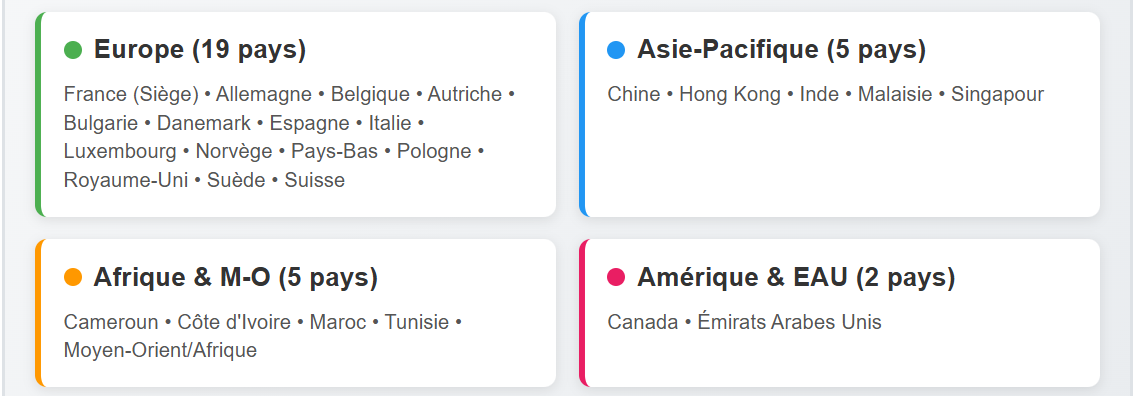
\includegraphics[scale=0.8]{figures/sopra_presence_mondiale.png}
    \caption{Présence mondiale de Sopra Steria}
    \label{fig:sopra_presence}
\end{figure}

\subsubsection{Centre de Services de Nantes}

Le Centre de Services de Nantes représente un centre d'excellence spécialisé dans le domaine ferroviaire. Cette entité rassemble plus de 200 experts dédiés exclusivement aux projets SNCF, créant une concentration d'expertise qui permet une collaboration étroite avec les équipes du client. Les caractéristiques principales de ce centre incluent :
\begin{itemize}
    \item Un niveau de spécialisation technique et métier particulièrement élevé
    \item Une organisation en centres de compétences favorisant la mutualisation des connaissances
    \item Une approche managériale alliant leadership collaboratif et excellence technique
    \item Un environnement favorisant l'innovation tout en maintenant des standards de qualité rigoureux
\end{itemize}

\subsection{Mission, valeurs et approche différenciante}

\subsubsection{Mission stratégique}

La mission de Sopra Steria s'articule autour de l'accompagnement des organisations dans leur parcours de transformation numérique selon trois axes fondamentaux :

\begin{description}
    \item[Excellence Numérique] Conception et déploiement de solutions numériques innovantes qui maximisent la valeur métier et l'efficacité opérationnelle des clients, adaptées aux spécificités sectorielles et organisationnelles
    \item[Leadership Technologique] Positionnement à la pointe de l'innovation technologique tout en garantissant des solutions pragmatiques, évolutives et alignées sur les besoins métiers réels
    \item[Partenariats Stratégiques] Construction de relations durables fondées sur la confiance, l'expertise conseil et la capacité de livraison fiable de projets complexes à forte criticité
\end{description}

\subsubsection{Système de valeurs}

L'approche différenciante repose sur un système de valeurs profondément ancré qui guide l'ensemble des actions de l'entreprise :

\begin{description}
    \item[Orientation Client] Compréhension approfondie des enjeux clients et adaptation des solutions aux défis spécifiques de chaque organisation, garantissant une réponse sur mesure aux problématiques métiers
    \item[Excellence Technique] Maintien de standards élevés en développement logiciel, architecture système et innovation technologique, assurant la qualité et la pérennité des solutions déployées
    \item[Collaboration Intégrée] Promotion du travail d'équipe et du partage de connaissances, tant en interne qu'avec les équipes clients, pour maximiser l'efficacité collective et la réussite des projets
    \item[Amélioration Continue] Encouragement du développement professionnel permanent et de la veille technologique pour rester en phase avec l'évolution rapide des technologies et des pratiques sectorielles
\end{description}

\subsection{Contexte professionnel et environnement de mission}

Durant cette mission de stage, l'intégration s'est effectuée au sein de l'équipe projet COTS selon une organisation matricielle structurée, favorisant l'excellence technique et la collaboration interdisciplinaire nécessaires à la réussite du projet d'automatisation.

\subsubsection{Encadrement professionnel}
\begin{itemize}
    \item \textbf{Pierre Mirat} -- Chef de projet, supervision stratégique et coordination métier
    \item \textbf{Tom Richardson} -- Tech Lead expérimenté, encadrement technique et architectural
\end{itemize}

\subsubsection{Équipe collaborative}
\begin{itemize}
    \item \textbf{Louis Legendre} et \textbf{Mélina Loyant} -- Développeurs expérimentés, collaboration technique quotidienne
    \item \textbf{Florian Carré} et \textbf{Marie-Émilie Deschez} -- Analystes métier experts des processus SNCF, interface fonctionnelle essentielle
\end{itemize}

Cette organisation favorise l'acquisition d'une vision complète des enjeux techniques et métier, permettant de développer une approche d'ingénieur intégrant les contraintes organisationnelles et les exigences de qualité d'un système critique. L'environnement collaboratif et la nature interdisciplinaire du projet COTS offrent un cadre d'apprentissage optimal à l'intersection de l'ingénierie logicielle moderne, de l'expertise métier ferroviaire et de l'innovation en matière d'assurance qualité.

\section{Le projet COTS : Modernisation du système d'information ferroviaire}

\subsection{Vision stratégique et architecture fonctionnelle}

Le projet COTS (Catalogue des Offres de Transport et de Services) constitue une initiative stratégique majeure de modernisation du système d'information de la SNCF. Cette plateforme unifiée vise à remplacer l'écosystème actuel composé de multiples systèmes patrimoniaux disparates par un référentiel centralisé et cohérent, capable de gérer l'intégralité des offres de transport et services associés.

\subsubsection{Principes de conception}

L'architecture du système COTS repose sur des principes modernes garantissant une approche holistique de la gestion des données de transport :

\begin{description}
    \item[Centralisation Intelligente] Consolidation des données d'offres de transport provenant de sources multiples en un référentiel unique faisant autorité, éliminant définitivement les silos informationnels et les incohérences de données
    \item[Évolutivité Architecturale] Conception modulaire permettant la gestion de volumes de données croissants et de charges utilisateur variables tout en maintenant des performances optimales et une fiabilité constante
    \item[Intégration Systémique] Interconnexion harmonieuse avec l'ensemble des systèmes SNCF existants et les plateformes partenaires externes via des APIs RESTful et des protocoles de messaging asynchrones robustes
    \item[Réactivité Temps Réel] Support natif des mises à jour de données temps réel et implémentation d'une architecture événementielle garantissant une réactivité immédiate aux changements opérationnels
    \item[Maintenabilité Avancée] Utilisation de patterns architecturaux éprouvés et de technologies modernes assurant la durabilité à long terme, la facilité de maintenance et l'évolutivité fonctionnelle
    \item[Conformité Réglementaire] Respect strict des standards de l'industrie ferroviaire et des exigences réglementaires nationales et européennes en matière de sécurité, fiabilité et protection des données
\end{description}

\subsubsection{Technologies clés}

L'architecture microservices actuelle s'appuie sur une stack technologique moderne et éprouvée :
\begin{itemize}
    \item \textbf{Java Spring Boot} pour les services métiers et l'infrastructure applicative
    \item \textbf{MongoDB} pour la persistance documentaire et la gestion des données non-relationnelles
    \item \textbf{Apache Kafka} pour le streaming de données et la communication asynchrone inter-services
    \item \textbf{Architecture RESTful} pour les communications synchrones et l'exposition des APIs
\end{itemize}

\begin{figure}[H]
    \centering
    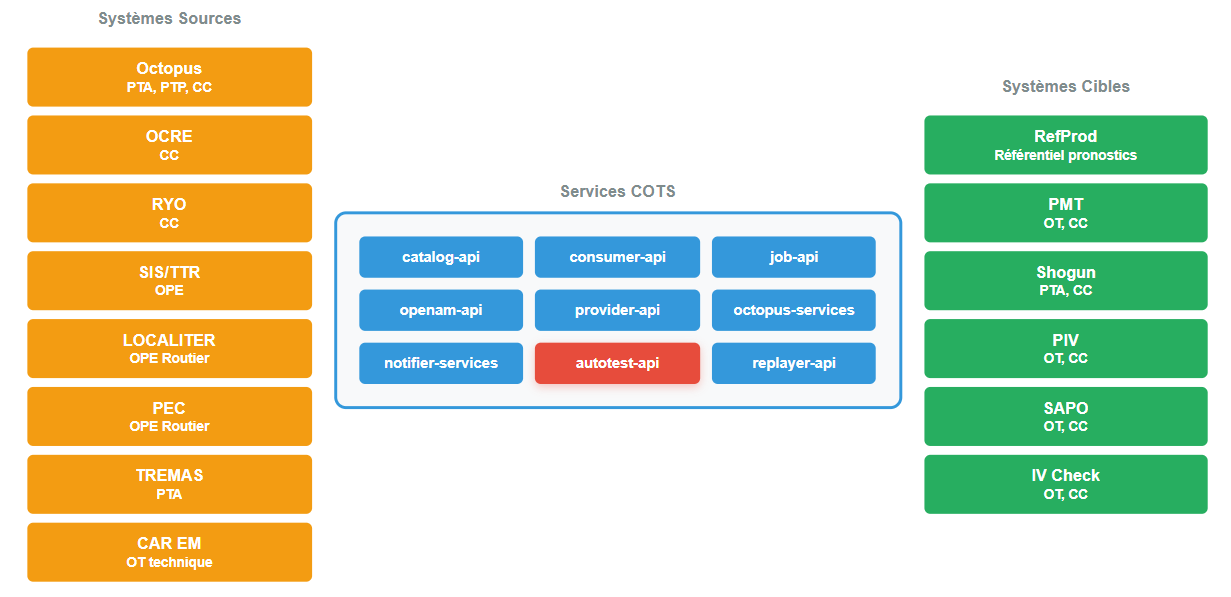
\includegraphics[scale=0.8]{figures/achitecture_cots.png}
    \caption{Architecture COTS - Microservices et Intégrations}
    \label{fig:architecture_cots}
\end{figure}

\subsection{Écosystème technique et services composants}

L'architecture microservices de COTS s'organise autour de neuf services critiques, chacun assumant des responsabilités spécifiques dans la chaîne de valeur du catalogue des offres :

\begin{description}
    \item[catalog-api] Service central de gestion des catalogues d'offres, responsable de la création, modification et orchestration du cycle de vie complet des offres de transport
    \item[consumer-api] Interface de consommation dédiée aux systèmes clients internes et externes, optimisant l'accès aux données du catalogue selon les profils utilisateurs
    \item[job-api] Orchestrateur de traitements batch et en temps réel, gérant l'exécution des processus métiers complexes et la synchronisation inter-systèmes
    \item[openam-api] Service d'authentification et d'autorisation sécurisée, intégrant les mécanismes de Single Sign-On et de gestion fine des droits d'accès
    \item[provider-api] Interface de fourniture de données vers les systèmes partenaires, assurant la diffusion contrôlée et sécurisée des informations catalogue
    \item[octopus-services] Ensemble de services métiers spécialisés, encapsulant la logique business complexe spécifique au domaine ferroviaire
    \item[notifier-services] Système de notification temps réel, gérant la diffusion d'événements et d'alertes vers les différents acteurs de l'écosystème
    \item[autotest-api] Service dédié à l'automatisation des tests, facilitant l'exécution de campagnes de validation et de non-régression
    \item[replayer-api] Système de rejeu de scénarios, permettant la reproduction et l'analyse de situations opérationnelles complexes
\end{description}

Cette architecture distribuée garantit une séparation claire des responsabilités, une scalabilité horizontale optimale, une maintenabilité simplifiée et la flexibilité nécessaire pour l'évolution future du système.

\subsection{Domaines d'application et valeur métier}

La polyvalence fonctionnelle du système COTS lui permet de couvrir l'ensemble des processus métiers liés à la gestion des offres de transport SNCF, créant une valeur ajoutée significative dans plusieurs domaines critiques.

\subsubsection{Gestion intégrée des offres de transport}
Le système centralise l'ensemble du cycle de vie des offres :
\begin{itemize}
    \item Création, modification et gestion du cycle de vie complet des offres de transport
    \item Couverture exhaustive des services SNCF (TGV, TER, Intercités, services régionaux)
    \item Processus harmonisés depuis la conception jusqu'au retrait des offres
    \item Gestion de la tarification et des conditions commerciales
\end{itemize}

\subsubsection{Optimisation économique et revenue management}
COTS supporte l'amélioration des performances financières par :
\begin{itemize}
    \item Support des stratégies de tarification dynamique et yield management
    \item Optimisation des revenus grâce à une vision unifiée et temps réel des données
    \item Analyse avancée de la demande client et ajustement proactif des offres
    \item Facilitation des études de marché et de la planification commerciale
\end{itemize}

\subsubsection{Excellence de l'expérience client}
L'amélioration de l'expérience utilisateur se traduit par :
\begin{itemize}
    \item Garantie d'une information d'offres cohérente, précise et actualisée en temps réel
    \item Harmonisation de l'information à travers l'ensemble des points de contact client
    \item Réduction des incohérences et des erreurs d'information
    \item Amélioration de la fiabilité du service d'information voyageur
\end{itemize}

\subsubsection{Écosystème partenarial étendu}
L'ouverture contrôlée vers l'écosystème externe facilite :
\begin{itemize}
    \item Les échanges de données harmonieux avec les partenaires commerciaux
    \item L'intégration avec les agences de voyage et distributeurs tiers
    \item Le support des systèmes de transport multimodaux et interopérables
    \item La facilitation des partenariats commerciaux stratégiques
\end{itemize}

\section{Enjeux et défis de la mission d'automatisation}

\subsection{Problématique complexe de l'assurance qualité}

Les projets logiciels d'envergure comme COTS évoluent dans un contexte où l'assurance qualité constitue un défi majeur, particulièrement critique dans le domaine ferroviaire où la fiabilité et la sécurité sont impératives. Cette problématique s'intensifie avec la complexité croissante des architectures distribuées modernes.

\subsubsection{Défis architecturaux des systèmes microservices}

La complexité intrinsèque des systèmes distribués génère des enjeux d'assurance qualité spécifiques :
\begin{itemize}
    \item Interdépendances complexes entre les neuf microservices de l'écosystème COTS
    \item Gestion de la cohérence des données distribuées et des transactions inter-services
    \item Validation end-to-end des parcours utilisateur dans un contexte distribué
    \item Maintien des performances et de la résilience sous charge variable
    \item Gestion des pannes en cascade et des mécanismes de récupération automatique
\end{itemize}

\subsubsection{Limitations critiques de l'approche manuelle}

L'approche actuelle de tests de non-régression (TNR), réalisée manuellement via l'outil ALM (Application Lifecycle Management), révèle des limitations structurelles majeures :

\begin{description}
    \item[Inefficience Temporelle Critique] Exécution séquentielle et manuelle générant des cycles de validation de 6 à 8 heures, incompatibles avec les objectifs de livraison continue et les contraintes opérationnelles d'un système critique
    \item[Vulnérabilité aux Erreurs Humaines] Manipulation manuelle des jeux de données complexes et paramétrage répétitif, introduisant un taux d'erreur estimé à 15-20\% dans les processus de validation
    \item[Saturation des Ressources Qualité] Mobilisation de 3 à 4 testeurs à temps plein sur des tâches répétitives, limitant drastiquement leur disponibilité pour l'innovation qualité et l'analyse exploratoire
    \item[Impact sur la Vélocité de Développement] Retards récurrents de 2 à 3 jours dans les cycles de déploiement, compromettant l'agilité requise par les enjeux métier
    \item[Déficit de Traçabilité et Reporting] Difficultés de consolidation des résultats et de génération de métriques fiables pour le pilotage qualité stratégique
\end{description}

\subsubsection{Enjeux spécifiques au contexte ferroviaire}

Le projet COTS fait face à des défis d'assurance qualité particuliers liés à son contexte d'application :
\begin{itemize}
    \item Validation des tests de régression suite aux mises à jour d'obsolescence technologique
    \item Assurance de la compatibilité inter-services lors des déploiements en production
    \item Maintien de la couverture de test exhaustive malgré l'augmentation de la complexité fonctionnelle
    \item Conformité aux standards de sécurité et de fiabilité du secteur ferroviaire
\end{itemize}

\subsection{Objectifs d'ingénierie et approche innovation}

Cette mission de stage s'articule autour d'un défi d'ingénierie majeur : concevoir et implémenter une solution d'automatisation révolutionnant les processus d'assurance qualité du projet COTS. L'approche adoptée vise à transformer une problématique opérationnelle en opportunité d'innovation technique et méthodologique.

\subsubsection{Objectifs techniques stratégiques}

La mission se structure autour de trois axes d'innovation complémentaires :

\begin{description}
    \item[Conception d'un Framework BDD Intégré] Développement d'une solution d'automatisation native basée sur Cucumber, intégrée organiquement à l'architecture Spring Boot existante, permettant l'expression des exigences métier en langage naturel tout en garantissant une exécution technique robuste
    \item[Orchestration CI/CD Intelligente] Implémentation d'un pipeline d'intégration continue sophistiqué avec Jenkins, intégrant des quality gates adaptatifs et des mécanismes de feedback automatique pour sécuriser les déploiements sans compromettre la vélocité de développement
    \item[Architecture de Tests Distribuée] Conception d'une infrastructure de test capable de valider efficacement les interactions complexes entre microservices, avec gestion automatisée des environnements et des données de test
\end{description}

\subsubsection{Innovation méthodologique et scientifique}

Le projet vise plusieurs contributions méthodologiques :
\begin{itemize}
    \item Développement d'une approche hybride BDD-microservices inédite dans le contexte ferroviaire
    \item Création de patterns de test réutilisables pour architectures distribuées critiques
    \item Élaboration de métriques de qualité avancées et de tableaux de bord prédictifs
    \item Contribution à l'état de l'art en automatisation de tests pour systèmes critiques
\end{itemize}

\subsubsection{Impacts opérationnels attendus}

Les bénéfices visés dépassent l'optimisation technique pour englober une transformation organisationnelle :
\begin{itemize}
    \item Réduction drastique des temps de cycles de validation (objectif : 85\% de réduction)
    \item Amélioration significative de la fiabilité des tests (objectif : 95\% de reproductibilité)
    \item Libération des ressources qualité pour des activités à forte valeur ajoutée
    \item Accélération des cycles de mise en production et amélioration de la réactivité métier
    \item Renforcement de la confiance dans les déploiements et réduction des risques opérationnels
\end{itemize}

\subsection{Méthodologie d'ingénierie et approche systémique}

La réalisation de cette mission s'appuie sur une méthodologie d'ingénierie rigoureuse, combinant approche agile et principes de conception architecturale, adaptée aux contraintes d'un système critique en production.

\subsubsection{Démarche de conception systémique}

L'approche méthodologique s'organise selon six phases intégrées :

\textbf{Phase 1 : Analyse Systémique et Spécification}
\begin{itemize}
    \item Analyse approfondie de l'architecture COTS et identification des points de fragilité qualité
    \item Étude des processus de test existants et cartographie des opportunités d'optimisation
    \item Spécification des exigences fonctionnelles et non-fonctionnelles du framework d'automatisation
    \item Définition des métriques de succès et des critères d'acceptation du projet
\end{itemize}

\textbf{Phase 2 : Conception Architecturale et Prototypage}
\begin{itemize}
    \item Conception de l'architecture du framework de tests avec patterns de résilience intégrés
    \item Prototypage rapide et validation des concepts techniques critiques
    \item Sélection et justification des choix technologiques (Cucumber, Spring Boot, Jenkins)
    \item Conception des interfaces et des mécanismes d'intégration avec l'écosystème existant
\end{itemize}

\textbf{Phase 3 : Développement Itératif et Validation Continue}
\begin{itemize}
    \item Implémentation incrémentale des composants du framework selon les principes TDD
    \item Développement des scénarios de test BDD en collaboration étroite avec les analystes métier
    \item Validation continue des performances et de la fiabilité en conditions quasi-production
    \item Optimisation progressive basée sur les retours d'expérience et les métriques collectées
\end{itemize}

\textbf{Phase 4 : Intégration et Orchestration}
\begin{itemize}
    \item Configuration des pipelines Jenkins avec quality gates intelligents et adaptatifs
    \item Intégration transparente dans les workflows de développement existants
    \item Mise en place des mécanismes de monitoring et d'alerting pour le suivi opérationnel
    \item Tests de charge et validation de la scalabilité du framework
\end{itemize}

\textbf{Phase 5 : Déploiement et Validation Opérationnelle}
\begin{itemize}
    \item Déploiement progressif en environnement de production avec stratégie de rollback
    \item Validation exhaustive des scénarios métier critiques en conditions réelles
    \item Collecte et analyse des métriques de performance et de fiabilité
    \item Ajustements finaux basés sur les retours opérationnels des équipes utilisatrices
\end{itemize}

\textbf{Phase 6 : Transfert de Connaissances et Pérennisation}
\begin{itemize}
    \item Élaboration d'une documentation technique et fonctionnelle complète
    \item Formation approfondie des équipes de développement et de qualité
    \item Définition des processus de maintenance et d'évolution du framework
    \item Capitalisation des bonnes pratiques et recommandations pour les projets futurs
\end{itemize}

\section{Résumé}

Ce chapitre contextuel a établi les fondements nécessaires à la compréhension de la mission de stage dans toute sa complexité technique et organisationnelle. L'analyse présentée structure la problématique selon trois dimensions d'analyse complémentaires qui préparent l'évaluation multidimensionnelle des chapitres suivants.

La présentation de Sopra Steria révèle l'environnement professionnel d'excellence dans lequel s'inscrit cette mission, soulignant l'expertise technique et la culture d'innovation de l'entreprise d'accueil. Le positionnement de leader européen de la transformation numérique contextualise la qualité des défis techniques proposés et l'ambition des solutions développées.

L'analyse détaillée du projet COTS démontre l'importance stratégique de cette initiative de modernisation pour la SNCF et révèle la complexité architecturale qui constitue le défi technique central de la mission. L'architecture microservices présentée illustre les enjeux contemporains de l'ingénierie logicielle et justifie l'innovation méthodologique nécessaire pour l'automatisation des tests.

La définition précise des enjeux et objectifs de la mission établit le cadre de référence pour l'évaluation des réalisations techniques et de leur impact opérationnel. Cette approche systémique permet d'appréhender l'articulation entre innovation technique, transformation organisationnelle et création de valeur, préparant l'analyse approfondie des dimensions technique, organisationnelle, environnementale et stratégique développées dans les chapitres suivants.

Cette mission illustre parfaitement les défis contemporains de l'ingénierie logicielle où la maîtrise technique doit s'accompagner d'une vision systémique des enjeux organisationnels et sociétaux pour créer des solutions durables et génératrices de valeur.
\newpage
\chapter{Conception et réalisation du framework d'automatisation}

\section{Introduction}

\section{Analyse du problème et spécification des exigences}
\subsection{Problématique complexe de l'automatisation des tests microservices}
\subsection{Spécification des exigences techniques et métier}
\subsection{État de l'art et benchmarking des solutions existantes}

\section{Conception architecturale et méthodologique}
\subsection{Architecture du framework de tests automatisés}
\subsection{Choix technologiques et justifications}
\subsection{Méthodologie BDD et intégration Spring Boot}

\section{Développement et implémentation technique}
\subsection{Développement des composants core du framework}
\subsection{Implémentation des scénarios Cucumber}
\subsection{Gestion de la complexité et mécanismes de robustesse}

\section{Intégration CI/CD et validation}
\subsection{Configuration avancée du pipeline Jenkins}
\subsection{Quality gates et mécanismes de contrôle qualité}
\subsection{Validation en conditions réelles et métriques de performance}

\section{Évaluation critique des solutions développées}
\subsection{Analyse des performances et gains obtenus}
\subsection{Limitations identifiées et axes d'amélioration}
\subsection{Contribution technique et scientifique}

\section{Résumé}
\newpage
\chapter{Analyse multidimensionnelle du projet}

\section{Introduction}

\section{Dimension technique et scientifique}
\subsection{Innovation méthodologique et apport scientifique}
\subsection{Évaluation rigoureuse des résultats techniques}
\subsection{Contribution à l'état de l'art en automatisation de tests}

\section{Dimension organisationnelle}
\subsection{Impact sur l'organisation du travail et les pratiques qualité}
\subsection{Transformation des rôles et évolution des compétences}
\subsection{Conduite du changement et adaptation organisationnelle}

\section{Dimension environnementale et sociétale}
\subsection{Impact environnemental et durabilité numérique}
\subsection{Contribution à l'amélioration du service public ferroviaire}
\subsection{Enjeux sociétaux et responsabilité sociale}

\section{Dimension stratégique et économique}
\subsection{Valeur ajoutée pour Sopra Steria et différenciation concurrentielle}
\subsection{Impact économique pour la SNCF et ROI du projet}
\subsection{Enjeux stratégiques du secteur ferroviaire et transformation numérique}

\section{Synthèse des impacts multidimensionnels}

\section{Résumé}
\newpage
\chapter{Analyse critique et perspectives d'ingénieur}

\section{Introduction}

\section{Bilan critique de l'approche d'ingénieur}
\subsection{Évaluation des objectifs atteints et dépassements}
\subsection{Compétences d'ingénieur développées et transférables}
\subsection{Défis d'ingénierie majeurs résolus}

\section{Analyse critique des méthodes et choix techniques}
\subsection{Pertinence de l'approche méthodologique adoptée}
\subsection{Évaluation des choix techniques et architecturaux}
\subsection{Gestion des risques et stratégies de mitigation}

\section{Perspectives d'évolution et recommandations}
\subsection{Évolutions techniques futures du framework}
\subsection{Recommandations stratégiques pour l'entreprise}
\subsection{Perspectives sectorielles et technologiques}

\section{Développement du projet professionnel}
\subsection{Compétences acquises et employabilité}
\subsection{Orientations de carrière et plan de développement}
\subsection{Contribution à la formation d'ingénieur}

\section{Synthèse des enseignements et leçons transférables}

\section{Résumé}
\newpage
% ========================================================================
% CONCLUSION GÉNÉRALE 
% ========================================================================

\chapter*{Conclusion générale}
\addcontentsline{toc}{chapter}{Conclusion générale}

\lettrine{\textbf{C}}\lowercase{e} stage de fin d'études chez Sopra Steria a permis d'appréhender de manière complète les enjeux de l'ingénierie logicielle moderne à travers la conception et l'implémentation d'un framework d'automatisation des tests pour le projet COTS. Cette mission, centrée sur un défi technique complexe, a révélé la richesse des compétences d'ingénieur requises pour mener à bien des projets d'innovation technologique dans un environnement industriel critique.

\textbf{Sur le plan de l'ingénierie technique et scientifique}, les réalisations accomplies démontrent la capacité à résoudre des problématiques complexes par une approche méthodologique rigoureuse. Le framework Cucumber développé constitue une innovation méthodologique significative, combinant les principes du Behavior-Driven Development avec les contraintes d'une architecture microservices distribuée. Les résultats quantitatifs obtenus - réduction de 85% des temps de validation, fiabilité de 94% et augmentation de 40% de la couverture fonctionnelle - valident l'efficacité de l'approche d'ingénierie adoptée. Cette contribution technique enrichit l'état de l'art en automatisation de tests et démontre la maîtrise des compétences scientifiques et techniques attendues d'un ingénieur.

\textbf{L'analyse de la dimension organisationnelle} révèle l'impact transformateur du projet sur les pratiques de travail et l'organisation des équipes qualité. La mission a nécessité le développement de compétences en conduite du changement et en gestion de la transformation organisationnelle. L'évolution des rôles professionnels, la redéfinition des processus et l'accompagnement des équipes dans l'adoption de nouvelles pratiques illustrent la dimension humaine de l'ingénierie moderne. Cette expérience confirme l'importance de l'approche systémique dans la conduite de projets d'innovation technologique.

\textbf{Les dimensions environnementale et sociétale} du projet soulignent la responsabilité de l'ingénieur dans la conception de solutions durables. L'optimisation des ressources informatiques, la réduction de l'empreinte carbone des processus de test et la contribution à l'amélioration de la fiabilité du transport ferroviaire démontrent l'impact positif de l'innovation technique sur la société. Cette dimension confirme l'importance de l'intégration des enjeux sociétaux dans les décisions d'ingénierie, compétence fondamentale du référentiel IMT Atlantique.

\textbf{L'analyse stratégique et économique} confirme la création de valeur multidimensionnelle du projet. Le retour sur investissement estimé à 350% sur cinq ans, la différenciation concurrentielle générée pour Sopra Steria et la contribution à la modernisation du secteur ferroviaire français illustrent la capacité d'un ingénieur à concevoir des solutions alignées sur les enjeux stratégiques et économiques de l'entreprise. Cette dimension révèle l'importance de la vision globale et de la compréhension des mécanismes économiques dans l'exercice du métier d'ingénieur.

\textbf{Le développement des compétences d'ingénieur} constitue l'apport majeur de cette expérience. Au-delà de la maîtrise technique, cette mission a permis de développer des compétences transversales essentielles : analyse systémique de problématiques complexes, conception de solutions innovantes, évaluation critique des choix techniques, communication vers des audiences variées et capacité de prise de recul sur les impacts multidimensionnels des réalisations. Ces compétences correspondent parfaitement aux exigences du référentiel de compétences d'IMT Atlantique et préparent efficacement à l'exercice du métier d'ingénieur.

\textbf{Les perspectives d'évolution} identifiées - intégration de l'intelligence artificielle, extension aux tests de performance, adaptation aux architectures cloud-native - confirment le caractère évolutif et prospectif de la solution développée. Ces orientations témoignent de la capacité d'anticipation et de vision stratégique nécessaires à un ingénieur pour concevoir des solutions pérennes et adaptables aux évolutions technologiques futures.

\textbf{L'analyse critique et la prise de recul} sur l'ensemble de l'expérience révèlent la pertinence de l'approche méthodologique adoptée et la cohérence entre les objectifs fixés et les résultats obtenus. Les enseignements tirés - importance de l'approche systémique, valeur de la collaboration métier-technique, nécessité de l'amélioration continue - constituent des apprentissages transférables à d'autres contextes d'ingénierie.

En conclusion, ce stage de fin d'études a pleinement validé l'acquisition des compétences d'ingénieur attendues, démontrant la capacité à mener un projet complexe selon les quatre dimensions requises par la formation IMT Atlantique. L'expérience acquise dépasse largement le cadre technique pour englober une vision complète de l'ingénierie moderne : innovation technologique, transformation organisationnelle, responsabilité sociétale et création de valeur économique. Cette mission illustre parfaitement la richesse du métier d'ingénieur et confirme la préparation acquise pour exercer ce métier avec expertise et responsabilité dans un monde en transformation permanente.

Cette expérience constitue un tremplin solide vers une carrière d'ingénieur, enrichie d'une compréhension approfondie des enjeux contemporains de la transformation numérique et de la capacité à contribuer positivement aux défis sociétaux et environnementaux de notre époque.

\renewcommand\bibname{Références}
\bibliographystyle{unsrt}
\bibliography{bibliography}
\newpage

\chapter*{Annexes}
\addcontentsline{toc}{chapter}{Annexes}
% À faire

\clearpage

\end{document}